%! Author = kyoto
%! Date = 11.09.2023

\vspace{3cm}
\tableofcontents

\newpage

\section{Задание}
Для каждого запроса предложить индексы, добавление которых уменьшит время выполнения запроса (указать таблицы/атрибуты, для которых нужно добавить индексы, написать тип индекса; объяснить, почему добавление индекса будет полезным для данного запроса).\\
Для запросов 1-2 необходимо составить возможные планы выполнения запросов. Планы составляются на основании предположения, что в таблицах отсутствуют индексы. Из составленных планов необходимо выбрать оптимальный и объяснить свой выбор.\\
Изменятся ли планы при добавлении индекса и как?\\
Для запросов 1-2 необходимо добавить в отчет вывод команды EXPLAIN ANALYZE [запрос]\\
Подробные ответы на все вышеперечисленные вопросы должны присутствовать в отчете (планы выполнения запросов должны быть нарисованы, ответы на вопросы - представлены в текстовом виде).\\

Сделать запрос для получения атрибутов из указанных таблиц, применив фильтры по указанным условиям:
\section{Запрос 1:}
\begin{verbatim}
    Таблицы: Н_ЛЮДИ, Н_СЕССИЯ.
    Вывести атрибуты: Н_ЛЮДИ.ОТЧЕСТВО, Н_СЕССИЯ.УЧГОД.
    Фильтры (AND):
    a) Н_ЛЮДИ.ОТЧЕСТВО > Александрович.
    b) Н_СЕССИЯ.УЧГОД < 2003/2004.
    Вид соединения: RIGHT JOIN.
\end{verbatim}

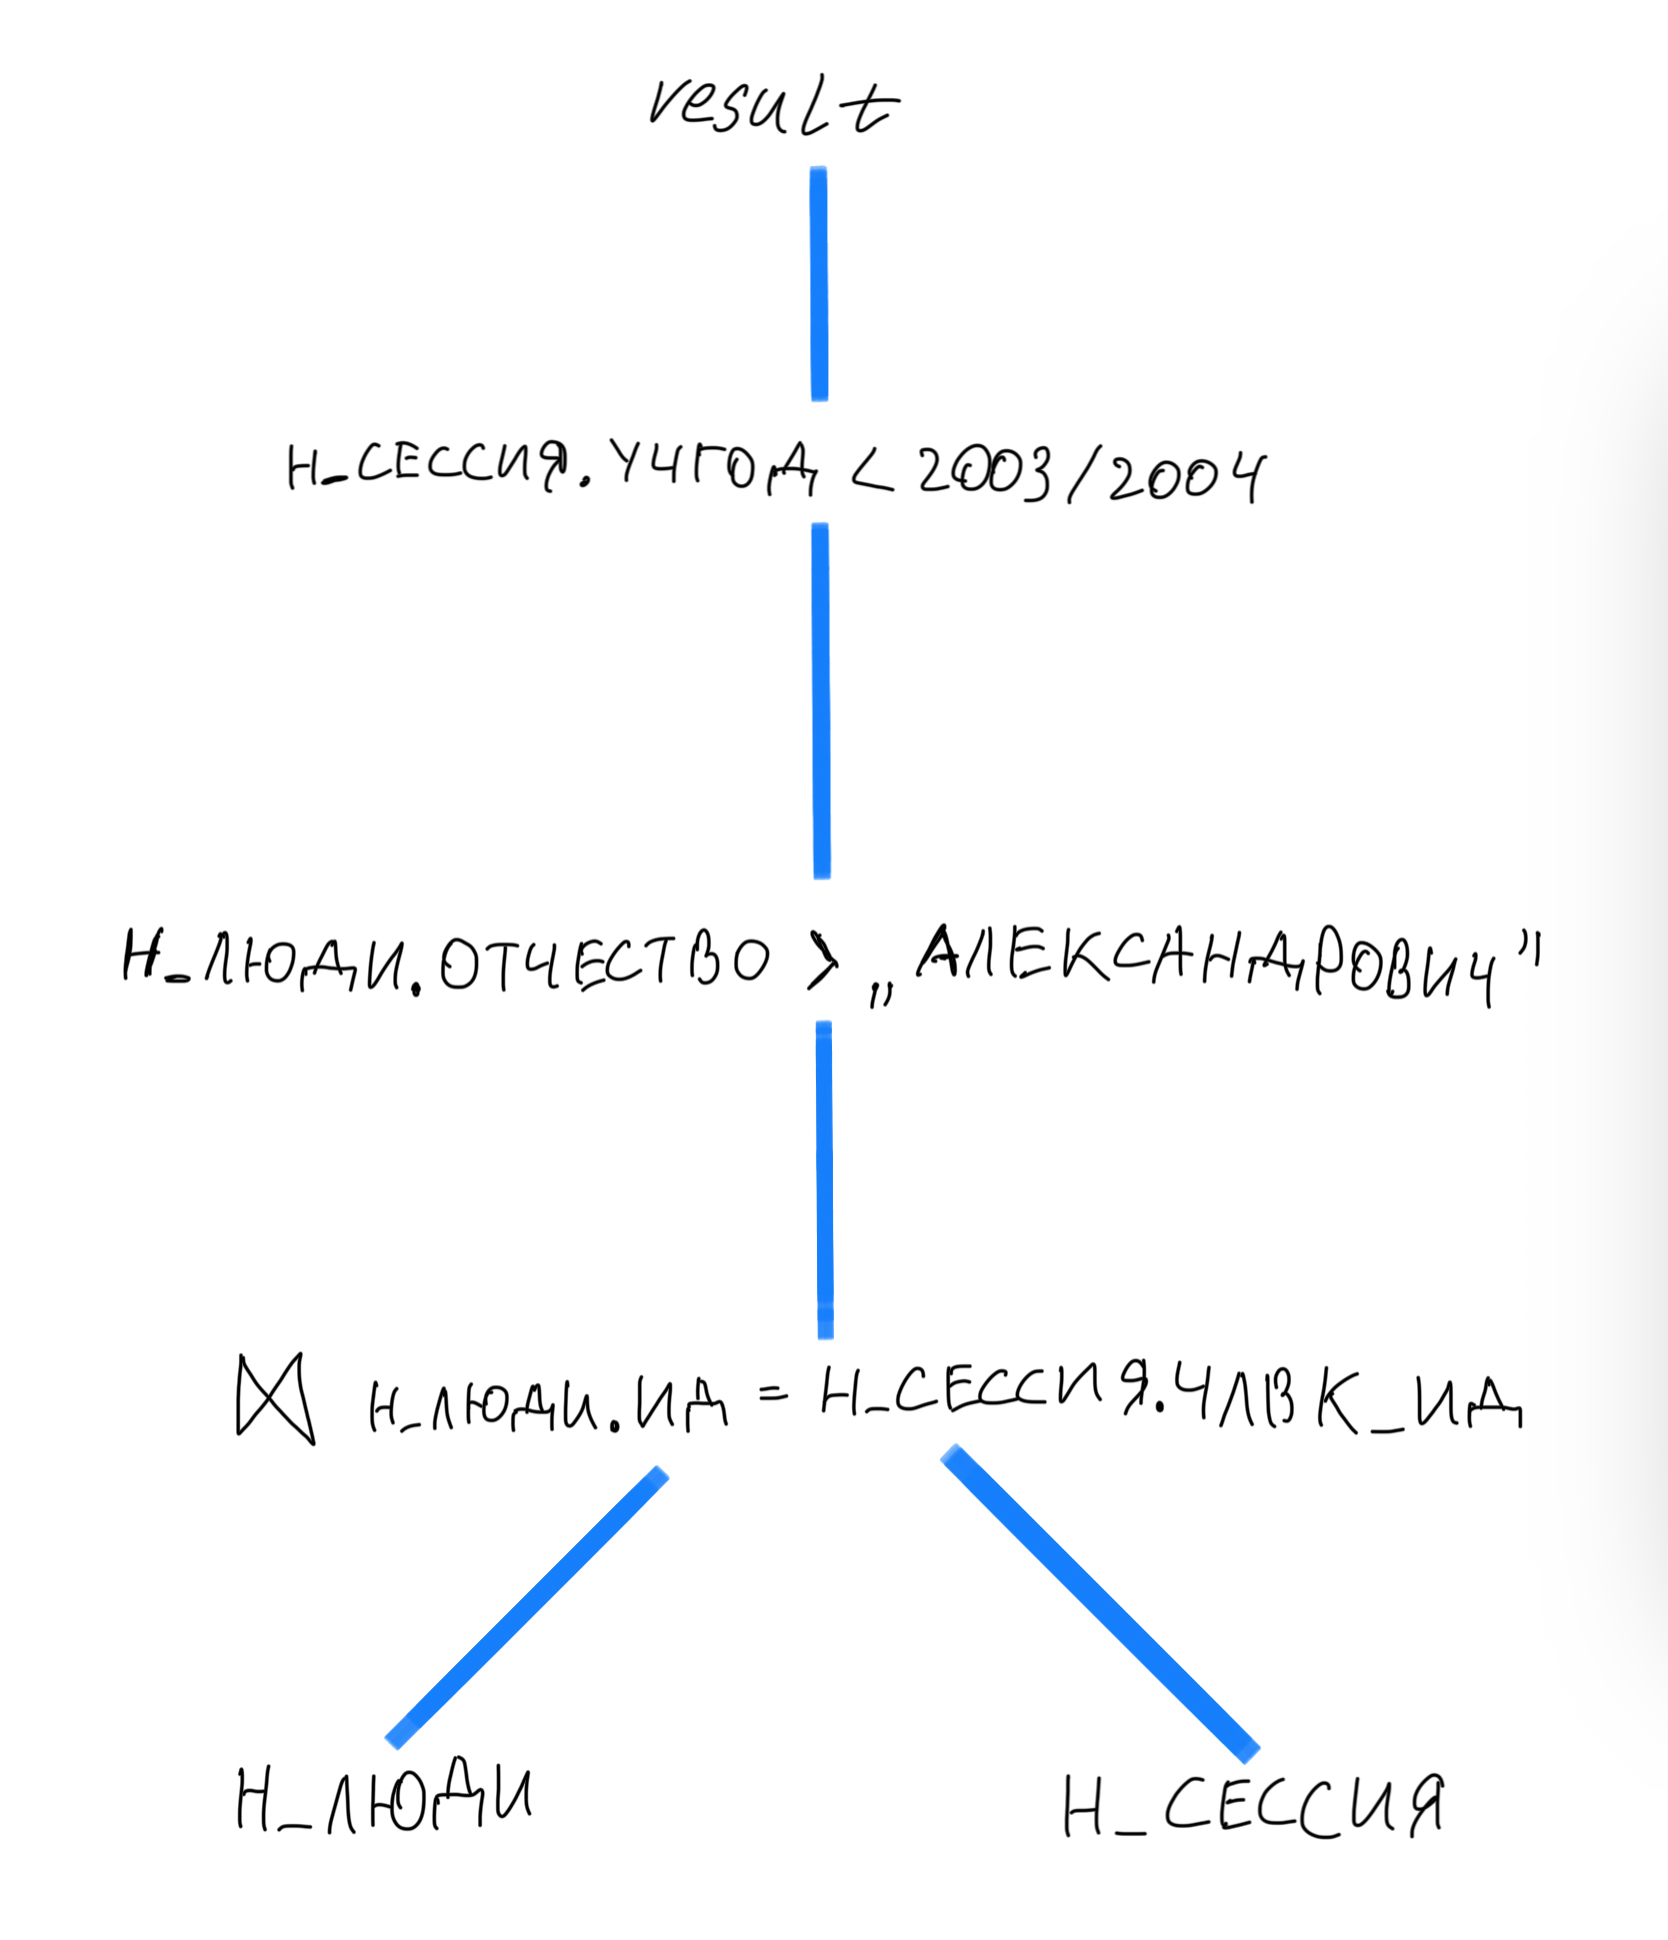
\includegraphics[scale=0.1]{img/3B458A37-05E0-4A86-8324-C65073974BD5_1_201_a}
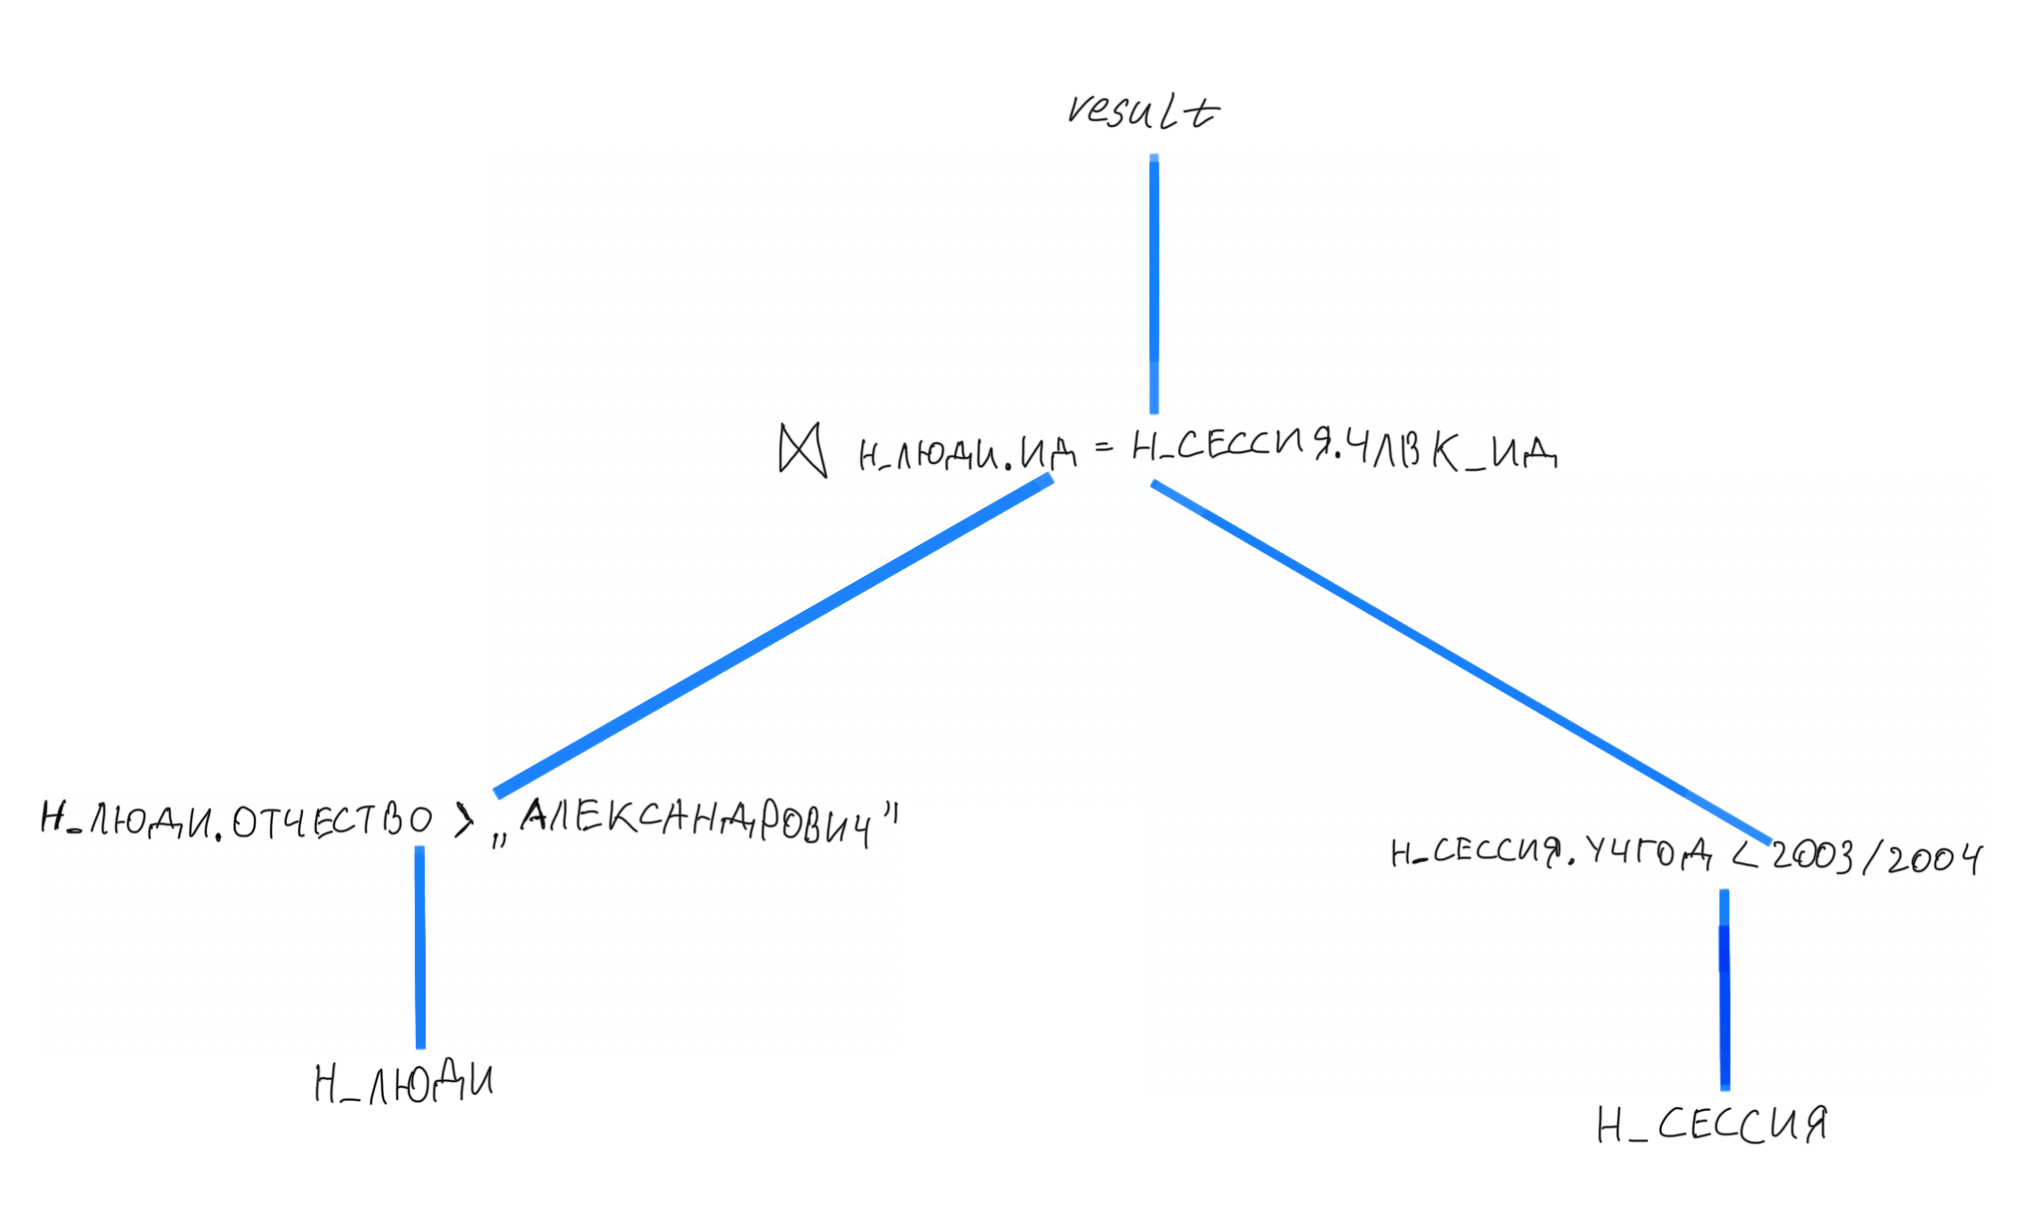
\includegraphics[scale=0.1]{img/8FA30A9A-F375-4B3C-B2FE-26DF1407B0A3_1_201_a}
Во втором плане происходит объединение только нужной выборки, а не всех сущностей. Размер промежуточных данных меньше, значит этот план является оптимальным.

\subsection{Предлагаемые индексы:}
так как выполняется сравнение при джоине, разумно использовать хэш на айдишниках, чтобы искать соответствие за O(1*)
\begin{verbatim}
    CREATE INDEX ON "Н_ЛЮДИ" USING HASH ("ИД");
    CREATE INDEX ON "Н_СЕССИЯ" USING HASH ("ЧЛВК_ИД");
\end{verbatim}

на полях, используемых для фильтров, оптимальным выбором будет индексация по бинарному дереву, так как идёт выборка по отношению порядка
\begin{verbatim}
    CREATE INDEX ON "Н_ЛЮДИ" USING BTREE ("ОТЧЕСТВО");
    CREATE INDEX ON "Н_СЕССИЯ" USING BTREE ("УЧГОД");
\end{verbatim}

\tiny
\begin{verbatim}
-----------------------------------------------------------------------------------------------------------------------
 Hash Join  (cost=218.21..337.05 rows=262 width=30) (actual time=4.282..5.739 rows=279 loops=1)
   Hash Cond: ("Н_СЕССИЯ"."ЧЛВК_ИД" = "Н_ЛЮДИ"."ИД")
   ->  Seq Scan on "Н_СЕССИЯ"  (cost=0.00..117.90 rows=358 width=14) (actual time=0.039..1.418 rows=358 loops=1)
         Filter: (("УЧГОД")::text < '2003/2004'::text)
         Rows Removed by Filter: 3394
   ->  Hash  (cost=163.97..163.97 rows=4339 width=24) (actual time=4.224..4.224 rows=4339 loops=1)
         Buckets: 8192  Batches: 1  Memory Usage: 314kB
         ->  Seq Scan on "Н_ЛЮДИ"  (cost=0.00..163.97 rows=4339 width=24) (actual time=0.008..3.474 rows=4339 loops=1)
               Filter: (("ОТЧЕСТВО")::text > 'Александрович'::text)
               Rows Removed by Filter: 779
 Planning Time: 0.460 ms
 Execution Time: 5.787 ms
\end{verbatim}

\normalsize

\section{Запрос 2:}
Сделать запрос для получения атрибутов из указанных таблиц, применив фильтры по указанным условиям:
\begin{verbatim}
    Таблицы: Н_ЛЮДИ, Н_ВЕДОМОСТИ, Н_СЕССИЯ.
    Вывести атрибуты: Н_ЛЮДИ.ОТЧЕСТВО, Н_ВЕДОМОСТИ.ЧЛВК_ИД, Н_СЕССИЯ.УЧГОД.
    Фильтры (AND):
    a) Н_ЛЮДИ.ИД = 152862.
    b) Н_ВЕДОМОСТИ.ДАТА = 2022-06-08.
    c) Н_СЕССИЯ.УЧГОД = 2008/2009.
    Вид соединения: RIGHT JOIN.
\end{verbatim}


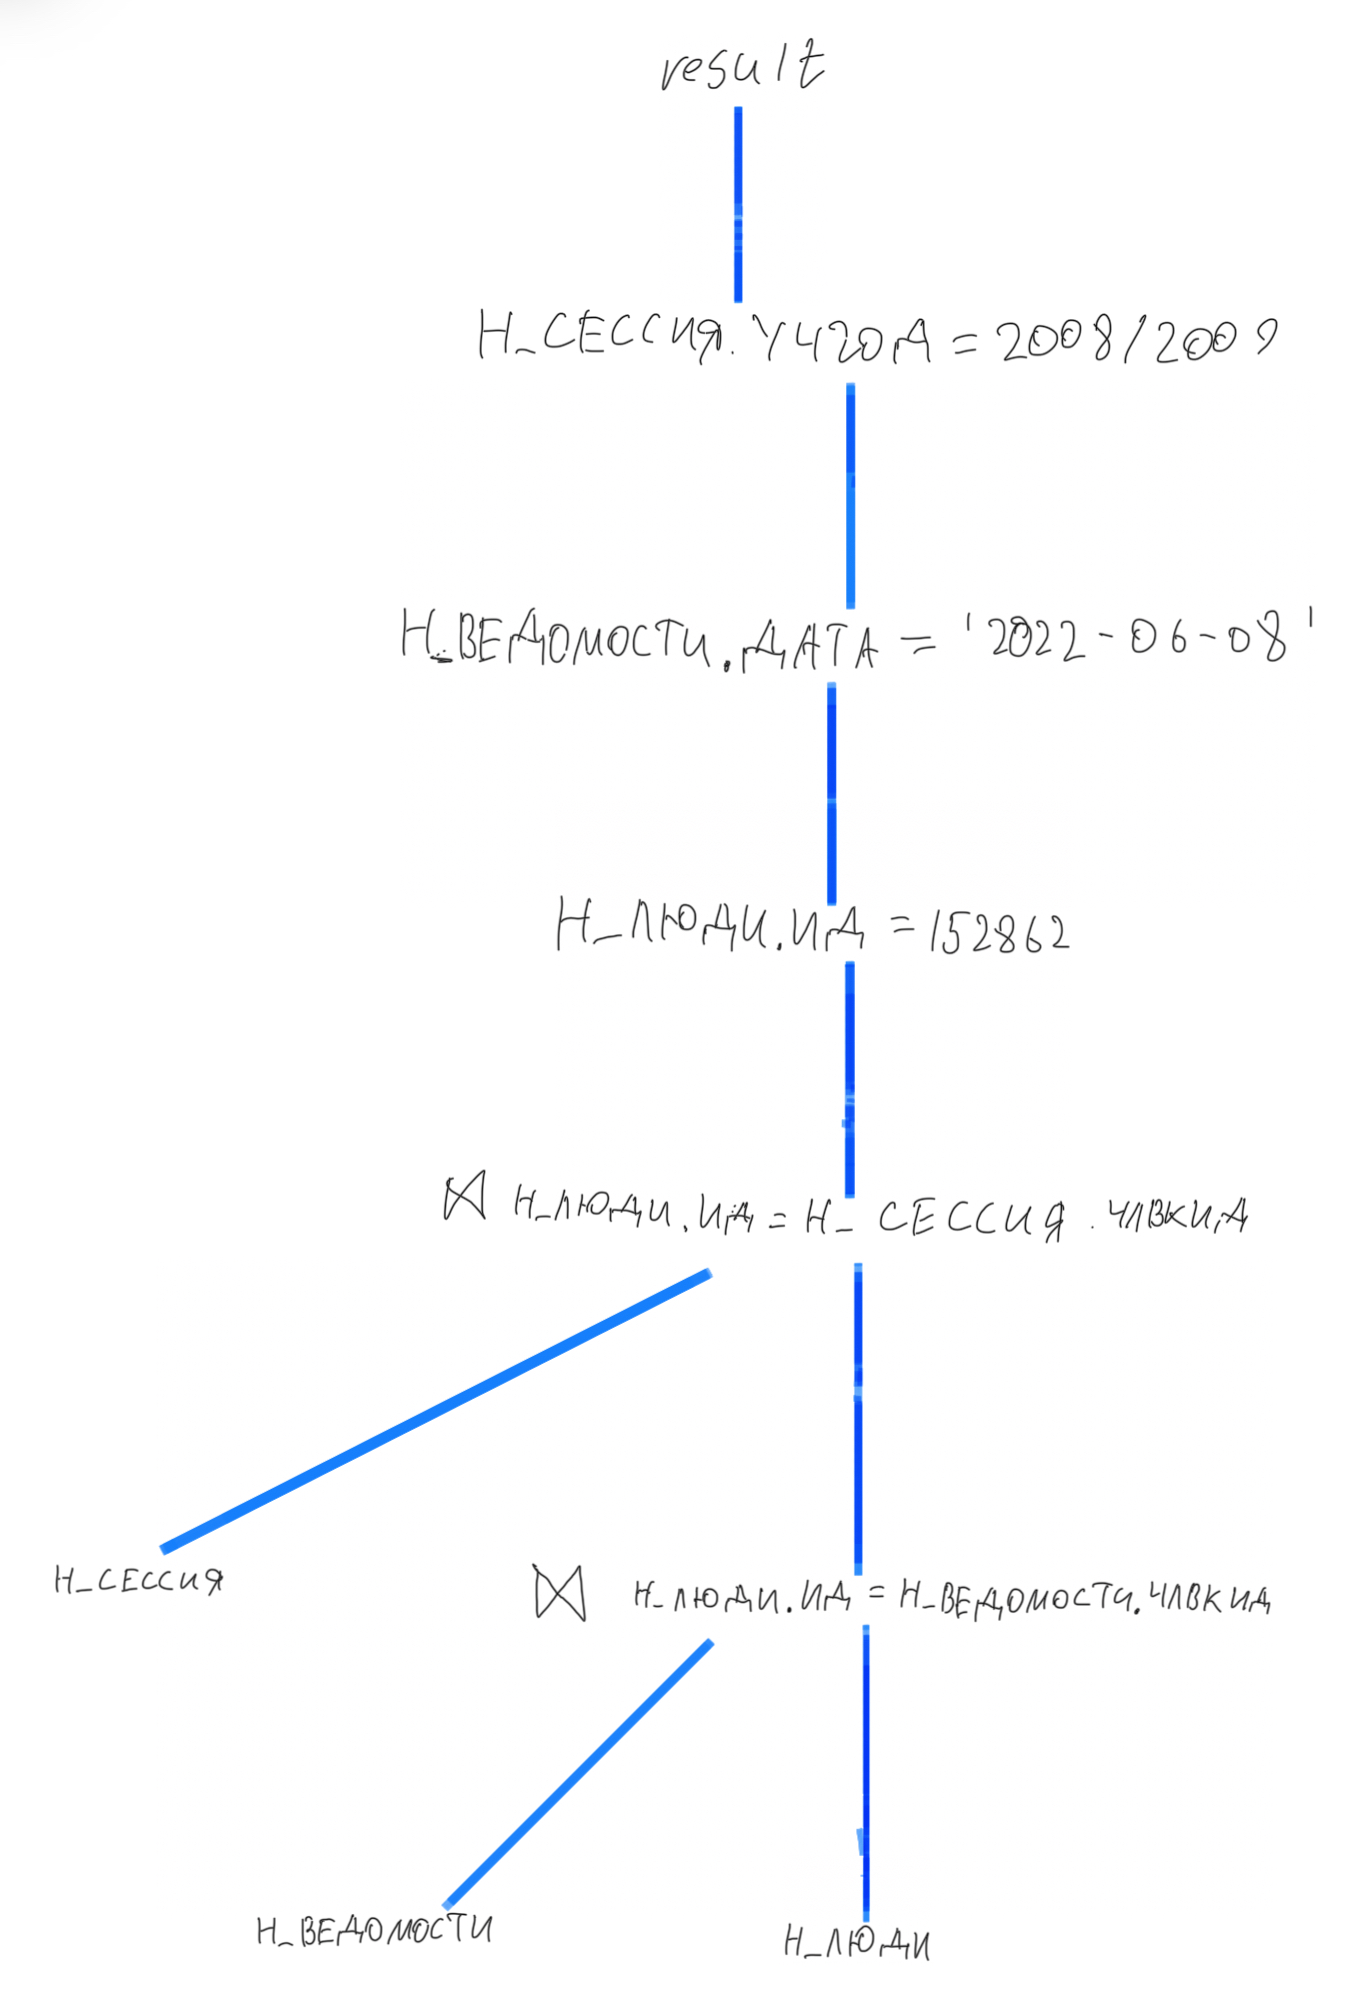
\includegraphics[scale=0.1]{img/3B3F657C-4110-4AE6-A736-745C403307F1_1_201_a}
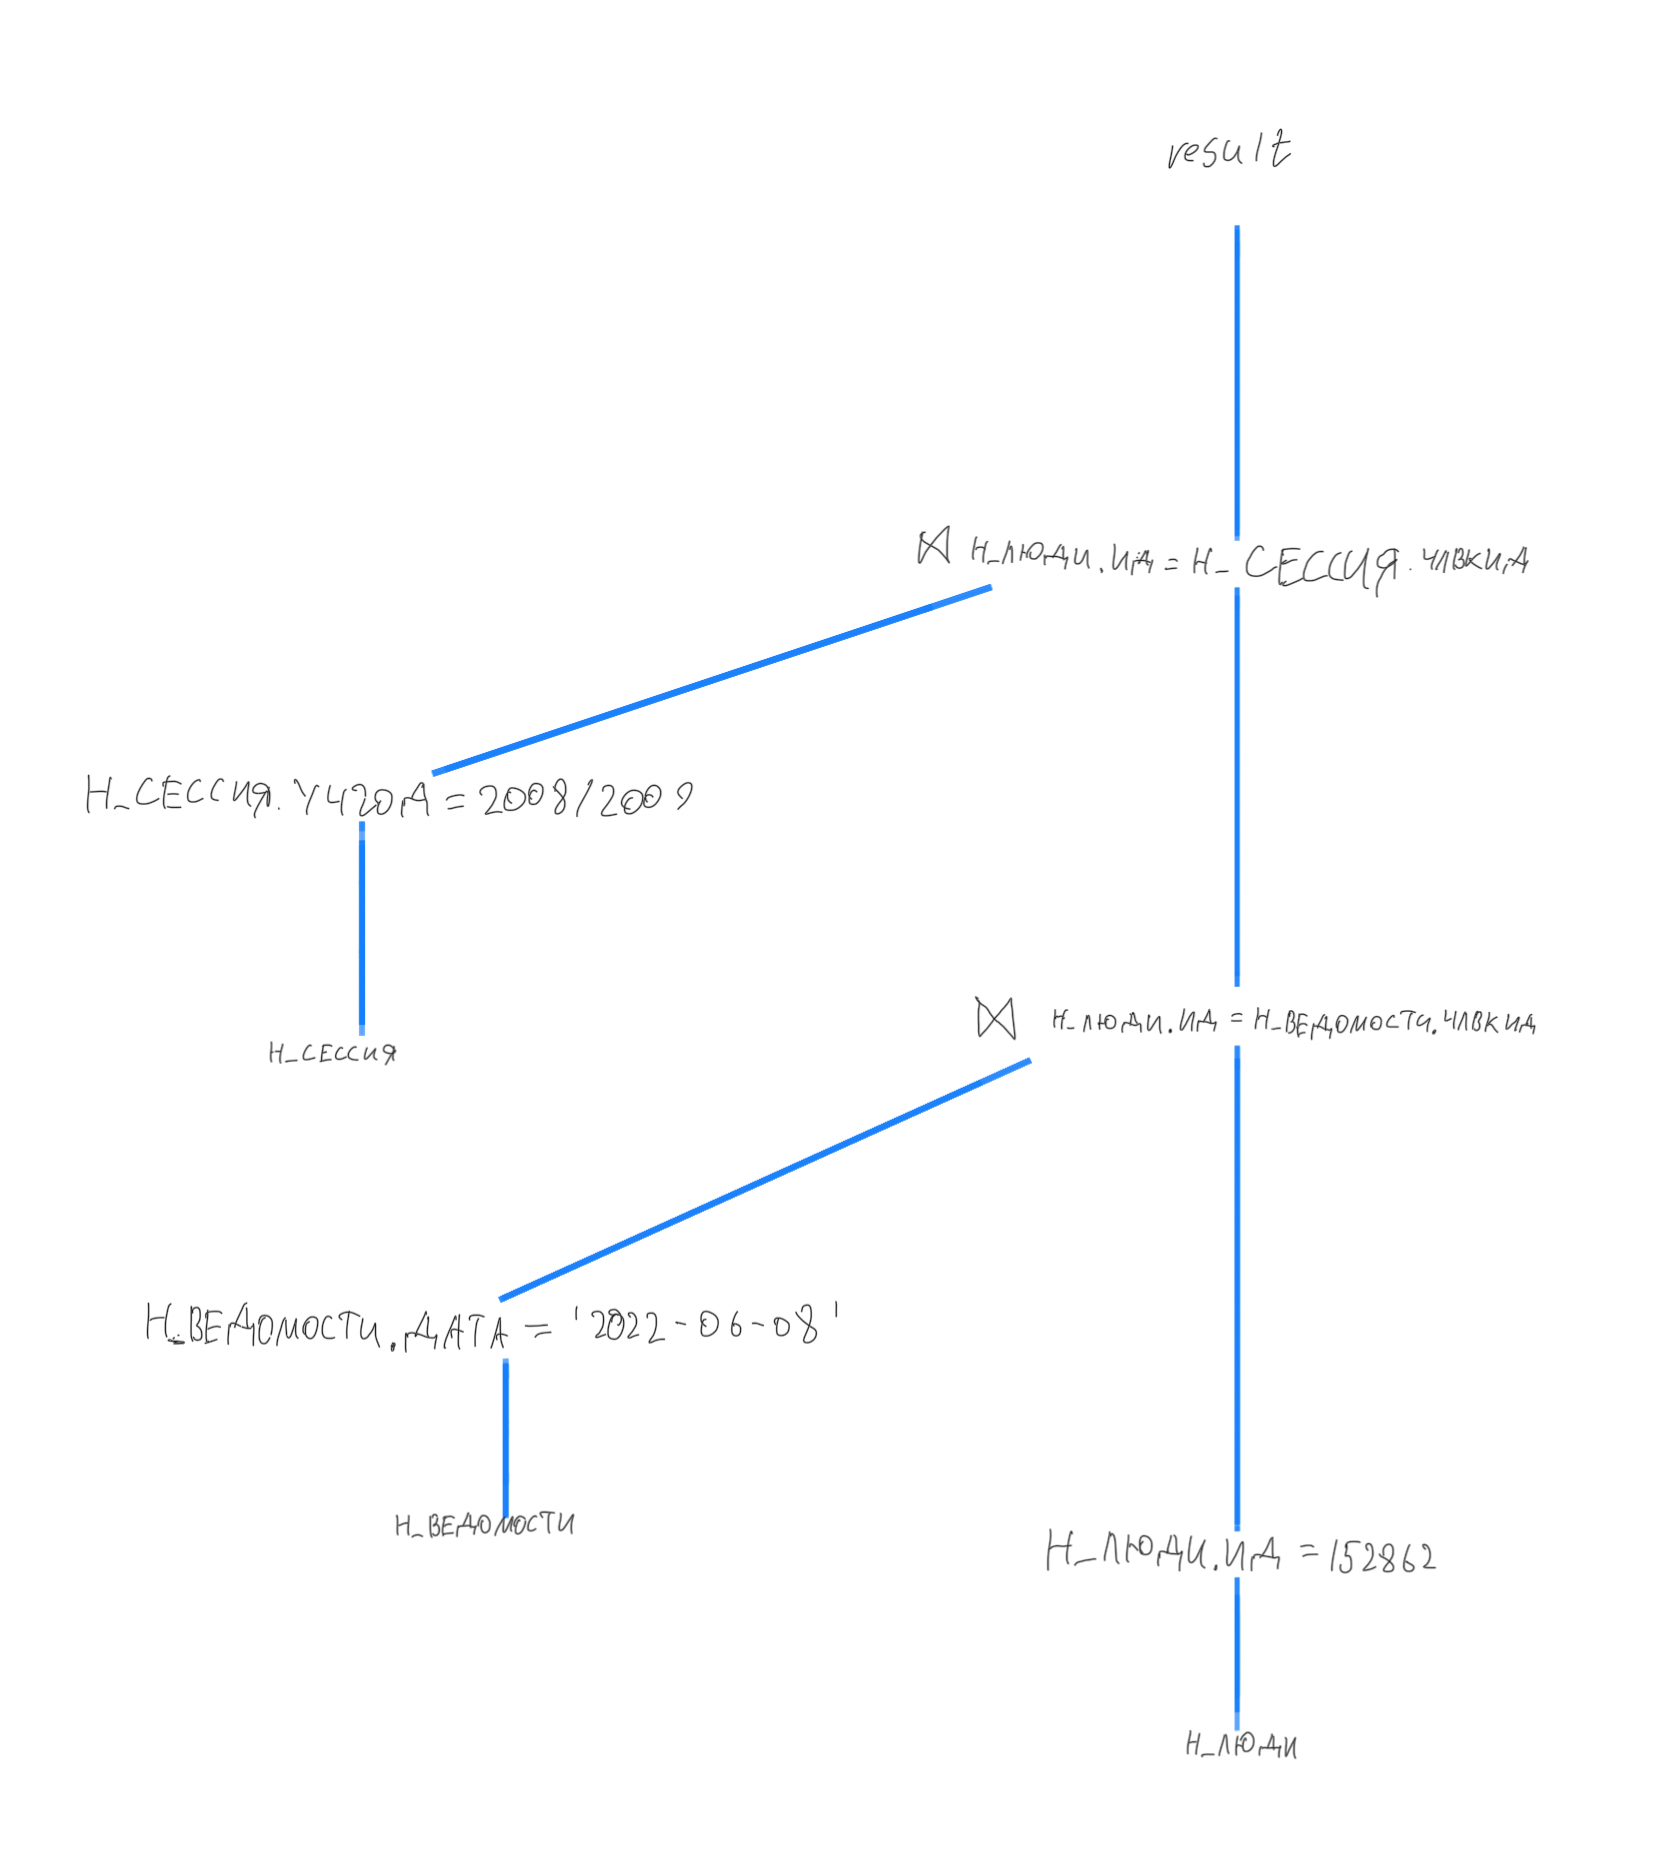
\includegraphics[scale=0.1]{img/1FE77B51-B421-4DC9-AFD1-15045EC0057A_1_201_a}
Во втором плане происходит объединение только нужной выборки, а не всех сущностей. Размер промежуточных данных меньше, значит этот план является оптимальным.
\subsection{Предлагаемые индексы:}
так как при джоине, и при фильтрации используется оператор сравнения, эффективнее будет индексировать по хэшу все значения
\begin{verbatim}
    CREATE INDEX ON "Н_ЛЮДИ" USING HASH ("ИД");
    CREATE INDEX ON "Н_СЕССИЯ" USING HASH ("ЧЛВК_ИД");
    CREATE INDEX ON "Н_ВЕДОМОСТИ" USING HASH ("ЧЛВК_ИД");
    CREATE INDEX ON "Н_ВЕДОМОСТИ" USING HASH ("ДАТА");
\end{verbatim}
\tiny
\begin{verbatim}
----------------------------------------------------------------------------------------------------------------------------------------------
 Nested Loop  (cost=14.45..33.52 rows=1 width=34) (actual time=0.076..0.078 rows=0 loops=1)
   ->  Nested Loop  (cost=10.15..22.19 rows=1 width=28) (actual time=0.076..0.077 rows=0 loops=1)
         ->  Index Scan using "ЧЛВК_PK" on "Н_ЛЮДИ"  (cost=0.28..8.30 rows=1 width=24) (actual time=0.013..0.013 rows=1 loops=1)
               Index Cond: ("ИД" = 152862)
         ->  Bitmap Heap Scan on "Н_ВЕДОМОСТИ"  (cost=9.87..13.88 rows=1 width=4) (actual time=0.058..0.058 rows=0 loops=1)
               Recheck Cond: (("ЧЛВК_ИД" = 152862) AND ("ДАТА" = '2022-06-08 00:00:00'::timestamp without time zone))
               ->  BitmapAnd  (cost=9.87..9.87 rows=1 width=0) (actual time=0.053..0.054 rows=0 loops=1)
                     ->  Bitmap Index Scan on "ВЕД_ЧЛВК_FK_IFK"  (cost=0.00..4.78 rows=65 width=0) (actual time=0.044..0.045 rows=43 loops=1)
                           Index Cond: ("ЧЛВК_ИД" = 152862)
                     ->  Bitmap Index Scan on "ВЕД_ДАТА_I"  (cost=0.00..4.83 rows=72 width=0) (actual time=0.005..0.005 rows=3 loops=1)
                           Index Cond: ("ДАТА" = '2022-06-08 00:00:00'::timestamp without time zone)
   ->  Bitmap Heap Scan on "Н_СЕССИЯ"  (cost=4.30..11.32 rows=1 width=14) (never executed)
         Recheck Cond: ("ЧЛВК_ИД" = 152862)
         Filter: (("УЧГОД")::text = '2008/2009'::text)
         ->  Bitmap Index Scan on "SYS_C003500_IFK"  (cost=0.00..4.29 rows=2 width=0) (never executed)
               Index Cond: ("ЧЛВК_ИД" = 152862)
 Planning Time: 0.697 ms
 Execution Time: 0.144 ms
\end{verbatim}                                                                  QUERY PLAN
